\documentclass[11pt, a4paper, twoside, openright]{article} %draft

%% Define the bibliography file to be used

\usepackage{graphicx,color}
\usepackage[backend=biber, style=numeric]{biblatex}
\usepackage{amssymb, amsmath, array}
\usepackage{listings}

\usepackage{booktabs}  % For \toprule, \midrule, \bottomrule
\usepackage{geometry}  % Optional, just for better margins
\geometry{margin=1in}

\addbibresource{citations.bib}



\begin{document}

% Example of title page for the projects carried out within the lasec 

% Simply include it in your mastex tex file: 
%        % Example of title page for the projects carried out within the lasec 

% Simply include it in your mastex tex file: 
%        % Example of title page for the projects carried out within the lasec 

% Simply include it in your mastex tex file: 
%        \input{cover}


% Updated March 2006 (SP)


\newcommand{\logoepfl}[0]{
  \begin{center}
    
\includegraphics[width=4cm]{logo_epfl_coul.eps}
  \end{center}
  \vspace{0.3cm}
  \hrule
}
\newcommand{\logolasec}[0]{
  \vspace{1cm}
  \hrule
  \begin{center}
    
\includegraphics[width=4.5cm]{logo_lasec_coul.eps}
  \end{center}
}
\newcommand{\project}[1]{
  \begin{center}
    \large{#1}
  \end{center}
  \vspace{1cm}
}
\newcommand{\department}[1]{
  \begin{center}
    \large{#1}
  \end{center}
}
\newcommand{\supervisor}[3]{
  \begin{center}
    \begin{normalsize}{
        \bf #1}\\#2\\#3
    \end{normalsize}
  \end{center}
}
\renewcommand{\author}[1]{
  \begin{center}
    \Large{#1}
  \end{center}
  \vspace{0.5cm}
}
\renewcommand{\title}[1]{
  \vspace{3cm}
  \begin{center}
    \huge{#1}
  \end{center}
  \vspace{1.7cm}
}
\renewcommand{\date}[2]{
  \begin{center}
    \normalsize{#1 #2}
  \end{center}
  \vspace{0.5cm}
}

\thispagestyle{empty}


% begin title page
  \logoepfl
  
  \title{An LLM-Based Taxonomy of Cultural Heritage Manipulation Detection: A Case Study on English Wikipedia Articles on Armenia}
  
  \author{Kaile Chu}
  \department{College of Digital Humanities}
  \project{Semester Project}
  
  \date{January}{2026}

  \begin{center}
    \begin{tabular}{cc}
      \begin{tabular}{p{4.0cm}}
        \supervisor{Responsible}{Prof. Frédéric Kaplan}{EPFL / DHLAB}
      \end{tabular}&
      \begin{tabular}{p{4.0cm}}
        \supervisor{Supervisor}{Emanuela Boros, Hamest Tamrazyan}{EPFL / DHLAB}
      \end{tabular}
    \end{tabular}
  \end{center}

% end title page
\clearpage




% Updated March 2006 (SP)


\newcommand{\logoepfl}[0]{
  \begin{center}
    
\includegraphics[width=4cm]{logo_epfl_coul.eps}
  \end{center}
  \vspace{0.3cm}
  \hrule
}
\newcommand{\logolasec}[0]{
  \vspace{1cm}
  \hrule
  \begin{center}
    
\includegraphics[width=4.5cm]{logo_lasec_coul.eps}
  \end{center}
}
\newcommand{\project}[1]{
  \begin{center}
    \large{#1}
  \end{center}
  \vspace{1cm}
}
\newcommand{\department}[1]{
  \begin{center}
    \large{#1}
  \end{center}
}
\newcommand{\supervisor}[3]{
  \begin{center}
    \begin{normalsize}{
        \bf #1}\\#2\\#3
    \end{normalsize}
  \end{center}
}
\renewcommand{\author}[1]{
  \begin{center}
    \Large{#1}
  \end{center}
  \vspace{0.5cm}
}
\renewcommand{\title}[1]{
  \vspace{3cm}
  \begin{center}
    \huge{#1}
  \end{center}
  \vspace{1.7cm}
}
\renewcommand{\date}[2]{
  \begin{center}
    \normalsize{#1 #2}
  \end{center}
  \vspace{0.5cm}
}

\thispagestyle{empty}


% begin title page
  \logoepfl
  
  \title{An LLM-Based Taxonomy of Cultural Heritage Manipulation Detection: A Case Study on English Wikipedia Articles on Armenia}
  
  \author{Kaile Chu}
  \department{College of Digital Humanities}
  \project{Semester Project}
  
  \date{January}{2026}

  \begin{center}
    \begin{tabular}{cc}
      \begin{tabular}{p{4.0cm}}
        \supervisor{Responsible}{Prof. Frédéric Kaplan}{EPFL / DHLAB}
      \end{tabular}&
      \begin{tabular}{p{4.0cm}}
        \supervisor{Supervisor}{Emanuela Boros, Hamest Tamrazyan}{EPFL / DHLAB}
      \end{tabular}
    \end{tabular}
  \end{center}

% end title page
\clearpage




% Updated March 2006 (SP)


\newcommand{\logoepfl}[0]{
  \begin{center}
    
\includegraphics[width=4cm]{logo_epfl_coul.eps}
  \end{center}
  \vspace{0.3cm}
  \hrule
}
\newcommand{\logolasec}[0]{
  \vspace{1cm}
  \hrule
  \begin{center}
    
\includegraphics[width=4.5cm]{logo_lasec_coul.eps}
  \end{center}
}
\newcommand{\project}[1]{
  \begin{center}
    \large{#1}
  \end{center}
  \vspace{1cm}
}
\newcommand{\department}[1]{
  \begin{center}
    \large{#1}
  \end{center}
}
\newcommand{\supervisor}[3]{
  \begin{center}
    \begin{normalsize}{
        \bf #1}\\#2\\#3
    \end{normalsize}
  \end{center}
}
\renewcommand{\author}[1]{
  \begin{center}
    \Large{#1}
  \end{center}
  \vspace{0.5cm}
}
\renewcommand{\title}[1]{
  \vspace{3cm}
  \begin{center}
    \huge{#1}
  \end{center}
  \vspace{1.7cm}
}
\renewcommand{\date}[2]{
  \begin{center}
    \normalsize{#1 #2}
  \end{center}
  \vspace{0.5cm}
}

\thispagestyle{empty}


% begin title page
  \logoepfl
  
  \title{An LLM-Based Taxonomy of Cultural Heritage Manipulation Detection: A Case Study on English Wikipedia Articles on Armenia}
  
  \author{Kaile Chu}
  \department{College of Digital Humanities}
  \project{Semester Project}
  
  \date{January}{2026}

  \begin{center}
    \begin{tabular}{cc}
      \begin{tabular}{p{4.0cm}}
        \supervisor{Responsible}{Prof. Frédéric Kaplan}{EPFL / DHLAB}
      \end{tabular}&
      \begin{tabular}{p{4.0cm}}
        \supervisor{Supervisor}{Emanuela Boros, Hamest Tamrazyan}{EPFL / DHLAB}
      \end{tabular}
    \end{tabular}
  \end{center}

% end title page
\clearpage



\tableofcontents
\clearpage

\section{Introduction}

\subsection{Motivation}

Cultural heritage and historical narratives are increasingly subject to deliberate manipulation in digital spaces. In this context, we use the term \textit{weaponization} to describe editorial interventions that subtly or overtly distort cultural, historical, or political narratives in order to advance a particular ideological position. Such manipulation may take the form of selective emphasis, strategic omission, terminological reframing, or emotionally charged language, and often operates beneath the threshold of overt vandalism. Unlike outright falsehoods, these tactics exploit ambiguity, framing, and perceived neutrality to influence interpretation while maintaining plausible deniability \cite{MORRISOCONNOR2022784}.

One of the platforms especially susceptible to this form of rhetorical contestation is Wikipedia. Although Wikipedia formally adheres to a non-partisan, neutral point-of-view (NPOV) editorial policy, this openness—while foundational to its collaborative model—has long been observed to foster editorial conflict, prolonged edit wars, and contested interpretations of what constitutes ``neutrality'' in practice \cite{MORRISOCONNOR2022784}. The policy’s flexibility can, in effect, provide substantial leeway for contributors to push articles toward ideologically slanted representations without necessarily violating explicit editorial rules. This susceptibility is further amplified by Wikipedia’s epistemic prominence. Articles from the English Wikipedia routinely appear at the top of search engine results and are widely treated as authoritative reference points. As a result, even subtle forms of content biasing can influence the historical understanding and political perceptions of vast numbers of English-speaking readers. In this sense, Wikipedia functions not merely as a passive repository of knowledge, but as an active battleground over cultural memory and narrative legitimacy.

Recent advances in natural language processing, particularly large language models (LLMs), have opened new avenues for studying such phenomena at scale. Recent prior work has demonstrated the potential of LLMs to detect rhetorical framing techniques in general such as in TV shows \cite{Alonso_del_Barrio_2024}, as well as political bias in more sensitive cultural/historical contexts such as news headlines or articles, with LLM-obtained conclusions largely agreeing with human annotators \cite{banik2025bridginghumanmodelperspectives}\cite{pastorino2024decodingnewsnarrativescritical}. However, much of this work remains focused on coarse-grained classification tasks in general and scarcely the domain of Wikipedia articles in particular, despite its similarities with news reports as informative and ostensibly neutral articles of media.

In this study, we thus focus on Wikipedia articles related to Armenia and Armenian culture and history. Armenia presents a particularly compelling case study due to its deep historical continuity and the persistence of unresolved geopolitical and historiographical disputes with neighboring states, most notably Turkey and Azerbaijan. The Armenian Genocide, widely recognized by historians as beginning in 1915, remains contested and denied in official Turkish discourse to this day. More recently, the 2020–2024 Azerbaijani offensives into Armenian-populated regions such as Nagorno-Karabakh have reignited intense narrative struggles over history, legitimacy, and cultural ownership. These dynamics create fertile ground for observing contemporary attempts at cultural and historical weaponization within a collaborative knowledge platform.

\subsection{Objectives}

The primary objective of this work is to investigate how an automated pipeline can be constructed to detect and categorize weaponized revisions related to Armenian cultural and historical heritage on the English Wikipedia. In particular, we evaluate the effectiveness of LLM-assisted approaches for identifying weaponization and distinguishing between manipulation techniques, in comparison to more traditional clustering- and topic-modeling-based methods. This study builds upon prior efforts by the EPFL DHLab to monitor cultural heritage weaponization on Wikipedia and its own deployment of LLMs in the pipeline \cite{hidri2025weaponization}, extending that work by more explicitly interrogating the feasibility of emergent versus predefined taxonomies.

Our findings indicate that while unsupervised clustering and topic modeling can partially surface thematic groupings, they struggle to cleanly separate weaponization techniques from article-specific content. In contrast, LLM-assisted analysis - particularly on the level of individual article edits/revisions - proves substantially more effective at both detecting weaponized edits and categorizing them into a refined ten-category taxonomy of manipulation techniques. Applying this framework further reveals systematic differences between Pro-Armenian and Anti-Armenian revision patterns, including asymmetric reliance on selective omission, insertion, and emotionally charged language, as well as a pronounced spike in weaponization activity around certain important points in time such as the 2020 Nagorno-Karabakh conflict.

Taken together, these results suggest that LLM-assisted revision-level analysis offers a promising new paradigm for monitoring cultural heritage manipulation on collaborative knowledge platforms, while also highlighting the limits of purely emergent taxonomic approaches in ideologically contested domains.

\subsection{Anticipated Challenges}

Prior to conducting this study, we anticipated several challenges that could complicate both detection accuracy and analytical interpretability. First, given the nuanced and often ambiguous nature of cultural heritage weaponization, we expected LLM-based judgments to exhibit nontrivial rates of misclassification, as is the case for any LLM-based task. Second, we anticipated that patterns in weaponization techniques - within the same year, across years, or between different stances - might be weaker or noisier than expected, potentially limiting our ability to drawn reliable conclusions regarding their characteristics. Most critically, we initially sought to avoid reliance on LLMs altogether—along with their associated opacity and accuracy concerns—by exploring whether traditional clustering and topic-modeling approaches could yield emergent taxonomies of weaponization techniques. However, we recognized the risk that such clusters, especially when derived from heterogeneous articles, might align more strongly with topical content than with manipulation strategies themselves. As demonstrated later in this study, this challenge proved to be the most consequential, directly motivating our eventual adoption of LLM-assisted, revision-level classification as a response to the limitations of purely unsupervised methods.


\section{Methodology}

Our unit of analysis is individual Wikipedia \textit{revisions} made to articles related to Armenian culture and history, along with the specific textual changes introduced by each revision. By focusing on revision-level diffs rather than article snapshots, we aim to capture fine-grained instances of narrative manipulation as they occur over time.

\subsection{Data Collection}

Both the data collection and first-stage weaponization detection steps are largely adapted from the previous DHLab study by Mohamed Hedi Hidri \cite{hidri2025weaponization}.

To capture a broad and representative cross-section of cultural and historical discourse, we began with a seed list of directly relevant categories, including ``Armenia,'' ``History of Armenia,'' and ``Culture of Armenia.''  From each seed category, we employed a two-layer recursive scraping procedure implemented in Python using \texttt{requests} and \texttt{BeautifulSoup}. For each page within a category, we retrieved the HTML of the main content area and extracted all in-article \texttt{/wiki/} links that did not belong to meta-namespaces (e.g., Talk, User, or Category pages). This process was then repeated once for the newly discovered subcategories as well as their own contained articles.

This procedure yielded a corpus of 925 articles spanning a wide range of topics, including historical events, religious institutions, political organizations, and cultural artifacts—domains particularly susceptible to ideological contestation and narrative manipulation.

For each selected article, we retrieved the complete revision history using the Wikimedia API’s \texttt{action=query} endpoint with \texttt{prop=revisions} and the parameter \\\texttt{rvprop=timestamp|user|comment|content}. Continuation tokens were handled programmatically to ensure exhaustive coverage of all revisions. Article states were reconstructed chronologically, and unified diffs between successive versions were computed using Python’s \\ \texttt{difflib.unified\_diff}.

To facilitate downstream processing by large language models, we further parsed each unified diff to explicitly extract added lines, removed lines, and word-level changes within modified lines. Each revision was stored as a JSONL record containing the raw diff hunks, structured fields for additions and deletions, and associated metadata (timestamp, editor identifier, and edit comment).

This data collection pipeline resulted in a total of 246{,}825 revisions across the 925 articles.

\subsection{First-Stage Weaponization Detection}

Our classification pipeline begins by framing each Wikipedia revision as a structured JSON object and tasking a large language model with reasoning directly over the observed textual changes. For each revision, we serialize either the full previous-version text or a diff-based representation—including the ISO timestamp, editor identifier, edit summary, and unified diff hunks—into a JSON snippet provided as model input.

At this stage, we employ \texttt{gpt-4o-mini}, selected due to its demonstrated remarkable classification accuracy in DHLab's prior work on detecting weaponized edits in articles related to the Russo–Ukrainian War \cite{hidri2025weaponization}, since the classification tasks in this study fundamentally iterate on those in the Russo-Ukrainian War study without substantially deviating from them. The model is instructed to assign exactly one of two labels: \texttt{Weaponised} or \texttt{Not Weaponised}, accompanied by a brief justification for its decision.

\lstset{
  basicstyle=\ttfamily\small, % Monospace font
  frame=single,
  breaklines=true, % Wrap long lines
  showstringspaces=false,
  tabsize=2
}

The prompt used for this classification step is as follows:

\begin{lstlisting}[frame=single]
2. For a revision (version "diff"):
   {{
     "version": "diff",
     "Timestamp": "<ISO timestamp>",
     "User": "<editor identifier>",
     "Comment": "<revision comment>",
     "Diff": "<original textual diff in unified diff format>"
     "Added_Lines": [<list of lines outright added>],
     "Removed_Lines": [<list of lines outright removed>],
     "Added_Words": [<list of words added in modified sentences>],
     "Removed_Words": [<list of words removed in modified sentences>]
   }}

  Important Instructions:
- If the version is "diff", focus primarily on the Added_Lines, Removed_Lines, Added_Words, and Removed_Words fields, i.e. on the lines (and words) actually added or deleted (i.e. not the lines that are untouched) as well as whatever additional context provided by the "User" and "Comment" fields.
- Ignore lines in the Diff field that have no prefix - these are unchanged context.
- Do not evaluate unchanged paragraphs for weaponization unless they were modified.
- For an original version (version "first_version"), treat it as baseline text.
- Analyze the text for subtle shifts in tone, style, or content that may be used to weaponize cultural heritage.

Below are examples of weaponisation terms and narratives:
- Term (Armenian Perspective):
  - "Armenian Genocide" (vs "alleged" or "disputed" genocide)
  - "Historical Armenian lands" / "Western Armenia"
  - "Cultural erasure of Armenians in Nakhichevan"
  - "Destruction of khachkars in Julfa"
  - "Ethnic cleansing of Armenians from Artsakh"
  - "Ancient Armenian monasteries in present-day Turkey"
  - "Armenian heritage sites under Azerbaijani control"
  - "Forced demographic changes in Nagorno-Karabakh"
- Term (Turkish/Azerbaijani/Rival Perspective):
  - "So-called Armenian Genocide"
  - "Turkish-Armenian relocation" / "1915 deportations"
  - "Caucasian Albanian heritage" (used to reattribute Armenian sites)
  - "Illegal occupation of Karabakh by Armenia"
  - "Liberation of Azerbaijani lands"
  - "Fabricated Armenian claims"
  - "Armenian aggression"
  - "Armenian terrorism" (used to describe ASALA/other groups)
  - "Destruction of Azerbaijani cultural sites by Armenians"
Implication or consequence: These terms may be used to justify actions, shift narratives, or frame cultural or territorial control in a specific light.

Using these examples as guidance, please provide a clear Judgment ("Weaponised" or "Not Weaponised" (if the change is grammatical, stylistic, or unrelated to cultural/political narratives)) along with a brief Explanation citing specific linguistic indicators from the "+" or "-" lines only.
Note that each entry might not strictly immediately follow prior ones, so only judge the entry by its own merit.

Here is the input JSON:
{record_json}

Your analysis:
\end{lstlisting}

To control computational cost, we restrict first-stage weaponization detection to a subdataset derived from the full corpus. Specifically, we select the 50 articles with the highest revision counts and randomly subsample 10\% of their revisions. This yields a final dataset of 12{,}659 revisions across 50 articles for in-depth analysis.

Each revision in this dataset is processed by the LLM to obtain both a binary weaponization judgment and an accompanying explanatory rationale, which are subsequently used in downstream analyses.



\subsection{Attempted Taxonomy Extraction via  Clustering/Topic Modelling}


Our initial major goal was to observe if the topics produced by clustering and/or topic modelling techniques alone are distinctive enough on the dimension of techinques to alone produce a clear taxonomy of weaponization techniques. 

As a first approach, we employ BERTopic, a widely used framework designed for topic modeling and clustering on textual corpora \cite{grootendorst2022bertopic}. More specifically, we adopt a customized variant of the standard BERTopic pipeline by customizing its submodules involving, respectively, sentence-level textual embedding, UMAP-based dimensionality reduction, and HDBSCAN clustering. UMAP projects high-dimensional embeddings (such as those obtained in this study) into a lower-dimensional space while preserving local neighborhood structure, and HDBSCAN identifies dense groups of semantically similar revisions while automatically labeling low-density points as noise. \cite{UMAP}\cite{HDBSCAN}
For textual embeddings, we use the HuggingFace sentence transformer model \texttt{Alibaba-NLP/gte-multilingual-base}\footnote{https://huggingface.co/Alibaba-NLP/gte-multilingual-base}, which produces 384-dimensional embedding vectors.

Rather than embedding the revision diffs themselves, we instead use the \textbf{LLM-generated explanations of weaponization judgments} themselves as input to the embedding stage. This design choice is motivated by the expectation that these explanations more directly encode information about the underlying weaponization techniques, as opposed to merely reflecting topical or subject-matter similarities present in the raw diffs.

For each subsidiary analysis discussed below, we perform a parameter sweep over the UMAP hyperparameters \texttt{n\_neighbors} (10, 20, 30, 40, 50, 60, 80, 120) and \texttt{n\_components} (5, 10, 15, 20), where \texttt{n\_components} denotes the dimensionality to which UMAP reduces the original embeddings. For each configuration, we select the optimal parameter combination based on silhouette scores, as well as qualitative assessments of whether the resulting number of clusters is interpretable and reasonable. To ensure reproducibility of the HDBSCAN clustering step, the \texttt{numpy} random seed is fixed at 42.


\subsection{Faction-Based Fine-Grained Analysis}

Finally, to further evaluate the LLM’s capacity for detecting and categorizing weaponized revisions, and to uncover potential systematic differences between opposing camps, we conduct an additional fine-grained analysis on all entries in the subdataset previously classified as \textit{Weaponized}. In this step, each weaponized revision is further categorized according to ideological stance as either \textit{Pro-Armenian} or \textit{Anti-Armenian}.

For clarity and to facilitate consistent interpretation by the LLM, we adopt expanded stance definitions. Specifically, \textit{Pro-Armenian} classifications are defined to also include revisions expressing anti-Turkish, anti-Azerbaijani, or otherwise oppositional stances toward historical rivals of Armenia. Conversely, \textit{Anti-Armenian} classifications also encompass revisions expressing pro-Turkish, pro-Azerbaijani, or otherwise favorable stances toward these same historical rivals.

These definitions are intended to capture the broader ideological alignment of each revision rather than narrowly construing stance as explicit pro- or anti-Armenian sentiment, thereby hopefully enabling more robust downstream analysis of factional patterns within weaponized edits.

The model used is once again \texttt{4o-mini}, and the prompt used for this step is as follows:
\begin{lstlisting}[frame=single]
You are an expert linguistic analysis assistant specializing in detecting subtle shifts in language that might be used to weaponize cultural heritage.

The input is a JSON record representing a Wikipedia article revision. The record follows this structure:
   {{
     "Source": "<original article name>",
     "Timestamp": "<ISO timestamp>",
     "User": "<editor identifier>",
     "Comment": "<revision comment>",
     "Diff": "<original textual diff in unified diff format>"
     "Added_Lines": [<list of lines outright added>],
     "Removed_Lines": [<list of lines outright removed>],
     "Added_Words": [<list of words added in modified sentences>],
     "Removed_Words": [<list of words removed in modified sentences>]
   }}

 Important Instructions:
- Focus primarily on the Added_Lines, Removed_Lines, Added_Words, and Removed_Words fields, i.e. on the lines (and words) actually added or deleted (i.e. not the lines that are untouched) as well as whatever additional context provided by the "User" and "Comment" fields.
- Ignore lines in the Diff field that have no prefix - these are unchanged context.
- Do not evaluate unchanged paragraphs for weaponization unless they were modified.
- Analyze the text for subtle shifts in tone, style, or content that may be used to weaponize cultural heritage.

Below are examples of weaponisation terms and narratives:
 Term (Pro-Armenian Perspective):
  - "Armenian Genocide" (vs "alleged" or "disputed" genocide)
  - "Historical Armenian lands" / "Western Armenia"
  - "Cultural erasure of Armenians in Nakhichevan"
  - "Destruction of khachkars in Julfa"
  - "Ethnic cleansing of Armenians from Artsakh"
  - "Ancient Armenian monasteries in present-day Turkey"
  - "Armenian heritage sites under Azerbaijani control"
  - "Forced demographic changes in Nagorno-Karabakh"
 Term (General Anti-Armenian aka Turkish/Azerbaijani/Rival Perspective):
  - "So-called Armenian Genocide"
  - "Turkish-Armenian relocation" / "1915 deportations"
  - "Caucasian Albanian heritage" (used to reattribute Armenian sites)
  - "Illegal occupation of Karabakh by Armenia"
  - "Liberation of Azerbaijani lands"
  - "Fabricated Armenian claims"
  - "Armenian aggression"
  - "Armenian terrorism" (used to describe ASALA/other groups)
  - "Destruction of Azerbaijani cultural sites by Armenians"
Implication or consequence: These terms may be used to justify actions, shift narratives, or frame cultural or territorial control in a specific light.

Using these examples as guidance, and - given that the given entry has already been judged as containing weaponization by a prior pipeline - please provide a clear Judgment (either "Pro-Armenian" or "Anti-Armenian") along with a brief Explanation citing specific linguistic indicators from the "+" or "-" lines only.
Special note that for the purpose of this analysis, "Pro-Armenian" can also encompass anti-Turkish or anti-Azerbaijani or anti-any-other-Armenian-historical-rival stances, while "Anti-Armenian" can also encompass pro-Turkish or pro-Azerbaijani or pro-any-other-Armenian-historical-rival stances.
Note that each entry might not strictly immediately follow prior ones, so only judge the entry by its own merit.

Here is the input JSON:
{record_json}

Your analysis:
\end{lstlisting}


\section{Results}

\subsection{Method 1: Taxonomy Extraction Attempt via Clustering with Custom Parameters}

Using the custom-parameter clustering pipeline described above, we obtain a total of 27 clusters. These clusters consist of \textbf{2572} revisions, having discarded \textbf{1392 (35.1\%)} out of the original \textbf{3964} revisions in the subdataset as noise. Based on silhouette score optimization and qualitative inspection, the optimal UMAP configuration was found to be \texttt{n\_neighbors = 10} and \texttt{n\_components = 20}. The resulting clusters are visualized in the left figure within Figure \ref{fig:combined} using a two-dimensional UMAP projection, illustrating a generally sufficient degree of semantic separation in the embedding space.

Below, we examine several representative clusters produced by this method. These case studies illustrate how individual clusters may—or, more often, may fail to—correspond cleanly to distinct weaponization techniques within a hypothetical taxonomy. For each cluster, we also report representative keywords extracted using \texttt{KeyBERT}, a tailor-made keyword extraction technique that leverages BERT embeddings to create keywords and keyphrases that are most similar to a given corpus \cite{grootendorst2020keybert}:

\begin{itemize}
\item \textbf{Cluster 0 (35 entries)}\\
\textit{(terms: action, territory, threat, terroristic, terrorism, distinction, context, nationalistic, oppression, heritage)}\\
Constituent revisions overwhelmingly concern the Armenian Revolutionary Federation (ARF, or Dashnaks), a major Armenian political organization historically involved in Armenian relations with external powers such as Ottoman authorities. These revisions frequently revolve around disputes over whether ARF activities constitute ``terrorism'' or whether the organization should be characterized as having ``conducted many terror acts against Turkish and Azeri communities,'' illustrating a blend of narrative framing and ideological contestation.

\item \textbf{Cluster 1 (1004 entries)}\\
\textit{(terms: teachgenocide, turkishness, heritage, weaponizing, holocaust, atrocity)}\\
At first glance, this cluster functions as a large ``big tent'' grouping. A substantial proportion of its constituent revisions concern the Armenian Genocide, particularly narrative, interpretive, and factual disputes surrounding the topic. However, beyond this shared subject matter, the cluster encompasses a wide range of editorial behaviors and weaponization techniques.

\item \textbf{Cluster 2 (49 entries)}\\
\textit{(terms: monument, wording, mausoleum, vandalise, propaganda, vandalised, preservation, weaponize, vandalism, artifact)}\\
Revisions in this cluster primarily involve accusations of cultural vandalism or erasure, often directed at Azerbaijani actors (and, in some cases, Armenian actors). Frequently cited sites include the Yukhari Govhar Agha Mosque and the Julfa Armenian cemetery, with edits disputing responsibility, intent, and framing of destruction or neglect.

\item \textbf{Cluster 3 (33 entries)}\\
\textit{(terms: aggressor, animosity, turkey, marginalize, provoke, demonize, linguistic, punitive, confrontational)}\\
Unlike many other clusters, Cluster 3 exhibits relatively weak thematic cohesion. Aside from a subset of revisions referencing ``a violent protest by Turks and Azeris against Armenians in Lyon, France,'' the dominant commonality lies in the use of extremely crude and emotionally charged language. Examples include additions or removals of phrases such as ``TAKE AWAY THE TURKISH FLAGS FROM THE GREEK ISLANDS !! SHAME ON YOU !! YOU ARE NOT OBJECTIVE !!!!'' and ``(Politically Lying Unholy Cowardly Killers).''

\item \textbf{Cluster 4 (83 entries)}\\
\textit{(terms: dish, arab, turks, delicacy, anatolia, assyrian, gastronomy, culinary, tolma, kurdish)}\\
This cluster is almost entirely centered on disputes surrounding the dish dolma, particularly competing claims over its cultural and national origins among Armenian, Azerbaijani, Lebanese, and other culinary traditions.
\end{itemize}

While a cluster such as Cluster 3 appears to be organized primarily along methodological lines, the above examples demonstrate that this is far from universally true. Many of the 27 clusters—including Clusters 0, 1, 2, and 4—are instead structured around a \emph{mixture} of weaponization techniques and topical or thematic content, rather than technique alone.

Cluster 1 is particularly illustrative of this limitation. Despite (or maybe because of, at a staggering 1004 entries) being the largest cluster, its only clear unifying feature is its focus on the Armenian Genocide. Within it, revisions span radically different weaponization strategies, ranging from the insertion of emotionally inflammatory headlines such as ``MASSACRE BY TURKS IN CAUCASUS TOWNS; Armenians Led Out Into the Streets and Shot or Drowned -- Old Friends Not Spared,'' to comparatively procedural edits involving the addition of maintenance tags such as \texttt{\{\{NPOV\}\}} and \texttt{\{\{Weasel section\}\}}.

Even Cluster 3, despite its small size (33 entries), exhibits internal heterogeneity. A subset of its revisions involve the removal of references to ``a specific incident where a group of Turks in Lyon, France, engaged in threatening behavior towards Armenians, including chanting derogatory phrases.'' These edits differ materially from other revisions in the same cluster that revolve around the insertion or deletion of emotionally charged or explicitly derogatory language. This relatively tangential connection around derogatory language likely explains why HDBSCAN grouped these revisions together.

Taken together, these observations suggest that clustering based solely on traditional clustering metrics (e.g., silhouette score) is insufficient for extracting clusters that are cleanly divided by weaponization technique. This tentatively reinforces the notion that assigning taxonomic labels at the level of \emph{individual revisions}, rather than retroactively inferring taxonomies from emergent clusters, may be a more viable strategy than initially anticipated.

This finding further motivates the exploration of alternative clustering-based approaches aimed at extracting a cleaner, technique-oriented taxonomy.

\subsection{Method 2: Taxonomy Extraction Attempt via Topic Modelling}

Applying BERTopic directly with default parameters yields a total of 69 topics. These topic-clusters consist of \textbf{2453} revisions, having discarded \textbf{1392 (38.1\%)} out of the original \textbf{3964} revisions in the subdataset as noise. Despite similar discard rates with the previous clustering approach (see Table \ref{tab:valid-noise-comparison} for a direct comparison), upon visualizing these topic-clusters in using once more a two-dimensional UMAP projection (as seen in the right figure of Figure \ref{fig:combined}), we can observe that microclusters in more diffuse spaces now exist compared to the previous clustering approach.

\begin{table}[h!]
\centering
\begin{tabular}{@{}lrr@{}}  % left-aligned, right-aligned, right-aligned
\toprule
\textbf{Category} & \textbf{Clustering} & \textbf{BERTopic} \\
\midrule
Total & 3964 & 3964 \\
Noise & 1392 (35.1\%) & 1511 (38.1\%) \\
``Valid'' Remaining & 2572 (64.9\%) & 2453 (61.9\%) \\
\bottomrule
\end{tabular}
\caption{``Valid'' revision counts and noise discard counts from the subdataset using both approaches}
\label{tab:valid-noise-comparison}
\end{table}

\begin{figure}[h!]
    \centering
    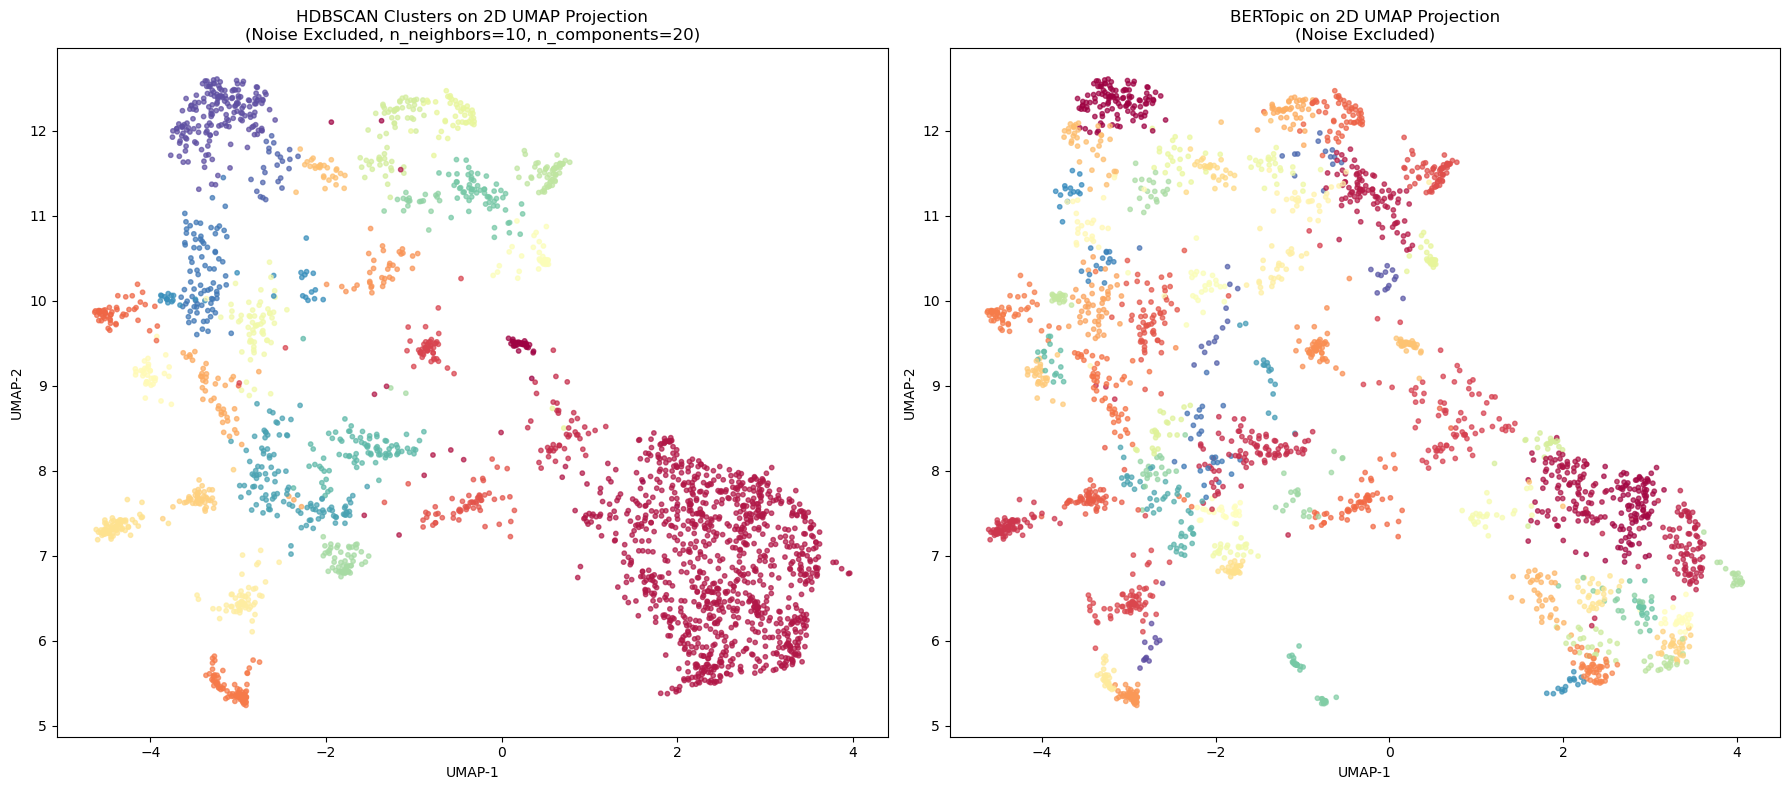
\includegraphics[width=1\linewidth]{fig/combined.png}
    \caption{Resulting topic-clusters via both approaches from Wikipedia Articles on Armenia, visualized on 2D}
    \label{fig:combined}
\end{figure}


Likewise, compared to the silhouette-score-based clustering approach, the ``big tent'' cluster problem is substantially alleviated. The largest topic produced by this method contains only 98 entries, a significant reduction from the 1004-entry cluster observed previously.

Moreover, this topic modeling pipeline demonstrates a noticeably improved ability to group revisions according to weaponization techniques rather than merely shared subject matter.

For instance, all entries assigned to Topic 53 concern removals of phrases, supporting materials such as ``a detailed report by former UN [personnel],'', or even entire sections from articles primarily focused on the Armenian Genocide.
\begin{itemize}
    \item Example: revision removing the detailed report by former UN Judge Geoffrey Robertson, which explicitly stated that there was an ``Armenian genocide'' and critiqued the British government's stance on the issue
    \item Example: revision removing the phrase ``In 2021, Labour MP John Spellar introduced a private members' bill to recognise the genocide, but the bill did not pass.'' which indicates a deliberate effort to downplay or erase the acknowledgment of the Armenian genocide within the context of UK parliamentary discussions
\end{itemize}

Similarly, Topic 41 consists exclusively of revisions involving the addition, removal, or replacement of Wikipedia maintenance templates such as \texttt{\{\{disputed\}\}} and \texttt{\{\{NPOV\}\}} in articles concerning the Armenian Genocide, and in one case, the Nagorno-Karabakh War.
\begin{itemize}
    \item Example: revision removing the tags \texttt{\{\{totallydisputed\}\}} and \texttt{\{\{inappropriate tone\}\}}, an act attempting to indicate a shift towards a more definitive stance on the topic of the Armenian Genocide
    \item Example: revision replacing the tag \texttt{\{\{POV\}\}} (indicating a ``Point of View'' concern) with \texttt{\{\{editag|Genocide Debate|NPOV\}\}} (indicating a ``Neutral Point of View'' within the context of a genocide debate), an act attempting to frame existant content in the article as neutral
\end{itemize}

The key insight from this second attempt is that weaponized edits \emph{can} be moderately separated by technique through clustering-based topic modeling, albeit imperfectly. However, this approach introduces its own limitations. A total of 69 topics may be excessive if the goal is to map each topic cleanly onto a single weaponization technique; it is not uncommon for individual weaponization techniques to be dispersed across multiple topics rather than consolidated within a single one. An example of this is revisions related to tag manipulation being present in both:
\begin{itemize}
    \item Topic 21, a revision removing the phrase "{{totallydisputed-section}}" from an article regarding the Armenian Revolutionary Federation (ARF) and its activities in Nagorno-Karabakh;
    
    And in:

    \item Topic 15: a revision appending a citation needed tag ({{Cn}}) to "Genocide." which implies an attempt to cast doubt on the established recognition of the Armenian Genocide.
\end{itemize}

Additionally, while topic modeling improves technique-level cohesion, clusters remain partially influenced by thematic content, indicating that this method does not entirely escape the content-driven biases observed in the first clustering approach.



\subsection{LLM-Assisted Manipulation Techniques Taxonomy Identification}

The clustering-based analyses presented above suggest that fully emergent taxonomies derived from unsupervised methods struggle to cleanly separate revision-based weaponization techniques from article-specific thematic content. While applying BERTopic with default parameters partially alleviates this issue, neither approach yields clusters that consistently align with discrete manipulation strategies. These findings motivate a shift away from retroactively inferring taxonomies from clusters, and toward the explicit construction of a technique-oriented classification framework.

Accordingly, we define a ten-category taxonomy to characterize the weaponization tactics employed by individual revisions. This taxonomy is adapted from the 17-category taxonomy employed in the previous DHLab study \cite{hidri2025weaponization}, but subsequently condensed following an initial survey of the revision entries in our dataset, with the goal of retaining only categories that are actually present in the dataset - with the possible exception of \textbf{Citation Washing} which appears extremely obscure in the dataset but we consider valuable to preserve regardless. Compared to the original taxonomy, category definitions have been refined to better reflect the forms of manipulation observed in practice. For each category, we provide an updated definition along with representative examples drawn directly from the dataset, as detailed below.
\begin{itemize}
    \item \textbf{Terminology Biasing}: Swapping neutral, or standard, or slanted-towards-one-side terms (for names, titles, exonyms, etc.) for alternatives culturally/ideologically slanted towards another side.
    \begin{itemize}
        \item Armenian Genocide vs. Armenian Relocation vs. so-called Armenian Genocide.
    \end{itemize}

    \item \textbf{Euphemism and Doublespeak}: Replacing direct language with softer phrasing to obscure meaning.
    \begin{itemize}
        \item Revision changing official state denial of the Armenian Genocide to that is considered by many historians as official state denial of the Armenian Genocide.
        \item Revision changing denying the Armenian Genocide to disputing the appropriateness of the Genocide label.
    \end{itemize}

    \item \textbf{Selective Omission}: Deleting inconvenient facts, dates, or events in the text proper to skew the narrative.
    \begin{itemize}
        \item Revision deleting a significant passage detailing the rounding up and imprisonment of Armenian intellectuals during the events of April 1915.
        \item Revision removing the line \texttt{[[Category:Genocides in Asia]]} from the Armenian Genocide article.
    \end{itemize}

    \item \textbf{Selective Insertion}: Adding one-sided or fringe claims/facts in the text proper that favor a particular agenda.
    \begin{itemize}
        \item Revision adding ===Websites supporting the genocide theses=== including an entire series of links to pro-Armenian websites.
        \item Revision claiming that No Turkish state official has visited Tsitsernakaberd.
    \end{itemize}

    \item \textbf{Source Biasing}: Replacing reputable citations with partisan ones (regardless of verifiability).
    \begin{itemize}
        \item Revision replacing a reference providing broader historical context with a citation to Dennis Papazian's book \emph{What Every Armenian Should Know}.
    \end{itemize}

    \item \textbf{Citation Washing}: Bulk-adding irrelevant or low-quality citations to fake credibility.
    \begin{itemize}
        \item Adding multiple low-quality sources (e.g., blogs, self-published sources, etc.) to support Turkish or Armenian claims.
    \end{itemize}

    \item \textbf{Citation Deletion}: Removing citations to make opposing views appear less verifiable.
    \begin{itemize}
        \item Removing a citation to Michael M.\ Gunter's work on Armenian Terrorism by labeling him a genocide denialist without evidence.
    \end{itemize}

    \item \textbf{Tag Manipulation}: Adding or removing Wikipedia tags to influence readers' perception of credibility or bias.
    \begin{itemize}
        \item Adding or removing neutral point of view tags on Armenian Genocide--related articles.
        \item Addition or removal of the \texttt{msg:TotallyDisputed} tag.
    \end{itemize}

    \item \textbf{Glorification \& Vilification}: Using loaded, emotionally appealing language to portray friendly subjects as heroic and opposing subjects as evil or barbaric.
    \begin{itemize}
        \item Revision claiming that Armenians were mean people and hated Americans.
        \item Revisions adding references to MASSACRE BY TURKS IN CAUCASUS TOWNS that emphasize Turkish atrocities while emotionally highlighting Armenian victimhood.
    \end{itemize}

    \item \textbf{Timeline Rewriting}: Shifting dates or sequences to alter causality or responsibility.
    \begin{itemize}
        \item Revision changing the Armenian Genocide date range from 1915--1916 to 1915--1922.
        \item Revision reframing the April 24, 1915 arrests of Armenian intellectuals from an event during the Armenian Genocide to the first major event of the Armenian Genocide.
    \end{itemize}
\end{itemize}




Out of all 3964 revisions judged as Weaponized, we obtain that 1761 are categorized as Pro-Armenian, 2199 are categorized as Anti-Armenian, and 4 revisions somehow escaped categorization (an ultimately negligible number that we nonetheless conservatively exclude from the two major categories). That is, Anti-Armenian edits slightly outnumber Pro-Armenian ones.

The final distribution of the different judgments on the entire 12659-revision dataset is visualized in Figure \ref{fig:piechart}.

\begin{figure}[h!]
    \centering
    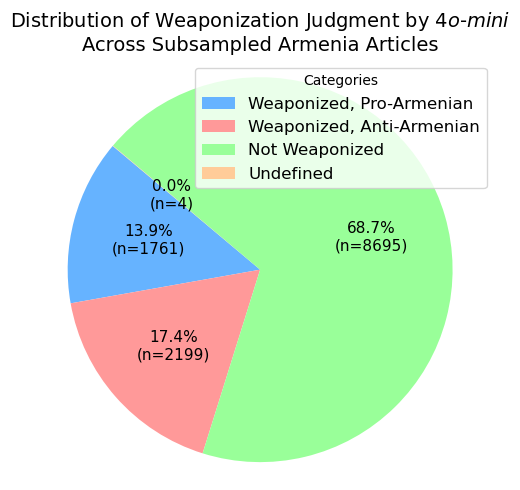
\includegraphics[width=0.7\linewidth]{fig/weaponization_cat_distr.png}
    \caption{Distribution of Weaponization Judgment by 4o-mini Across Subsampled Armenia Articles}
    \label{fig:piechart}
\end{figure}

\subsubsection{Patterns of Pro-Armenian vs Anti-Armenian Revisions over Time}

We can now plot out in Figures \ref{fig:barplot_three_direction} and \ref{fig:barplot_ratio} the year-wise fluctuation of both Pro-Armenian and Anti-Armenian revision count, as well as their respective percentages of each year's total edits, weaponized or not, (as a better reflection of the relative editorial activities from both camps), per year since Wikipedia's founding in 2001.

\begin{figure}[h!]
    \centering
    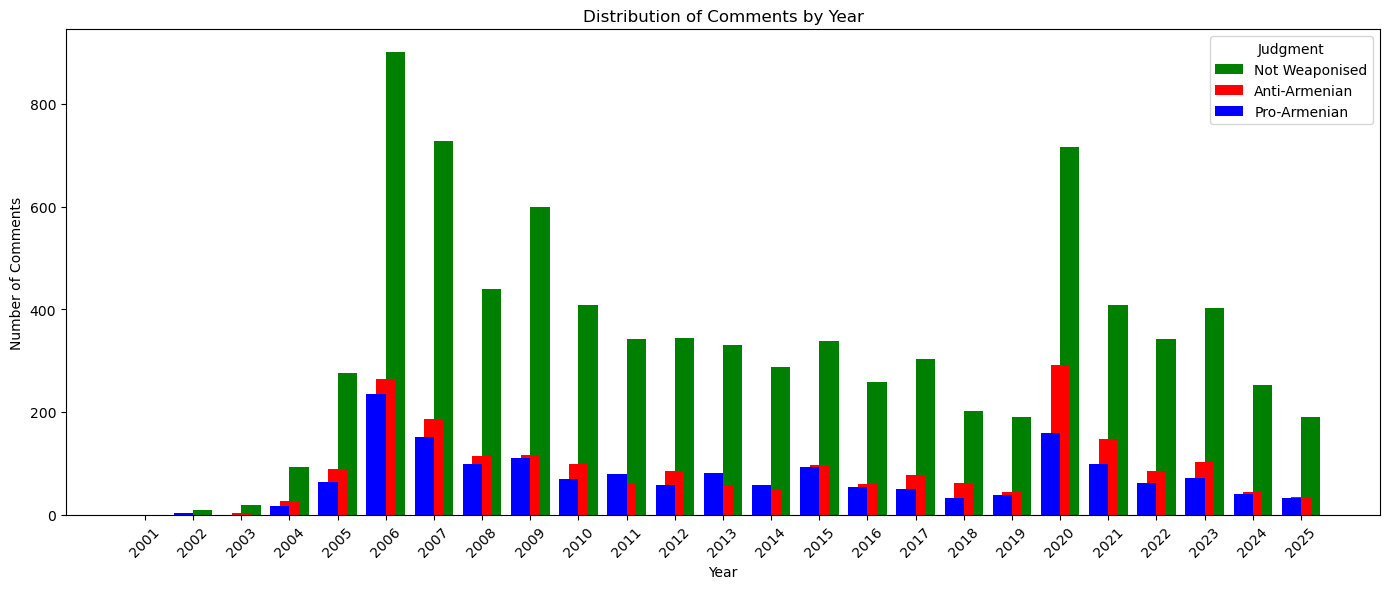
\includegraphics[width=0.8\linewidth]{fig/barplot_three_direction.png}
    \caption{Pro- And Anti-Armenian Revision Counts on English Wikipedia Over Time}
    \label{fig:barplot_three_direction}
\end{figure}

\begin{figure}[h!]
    \centering
    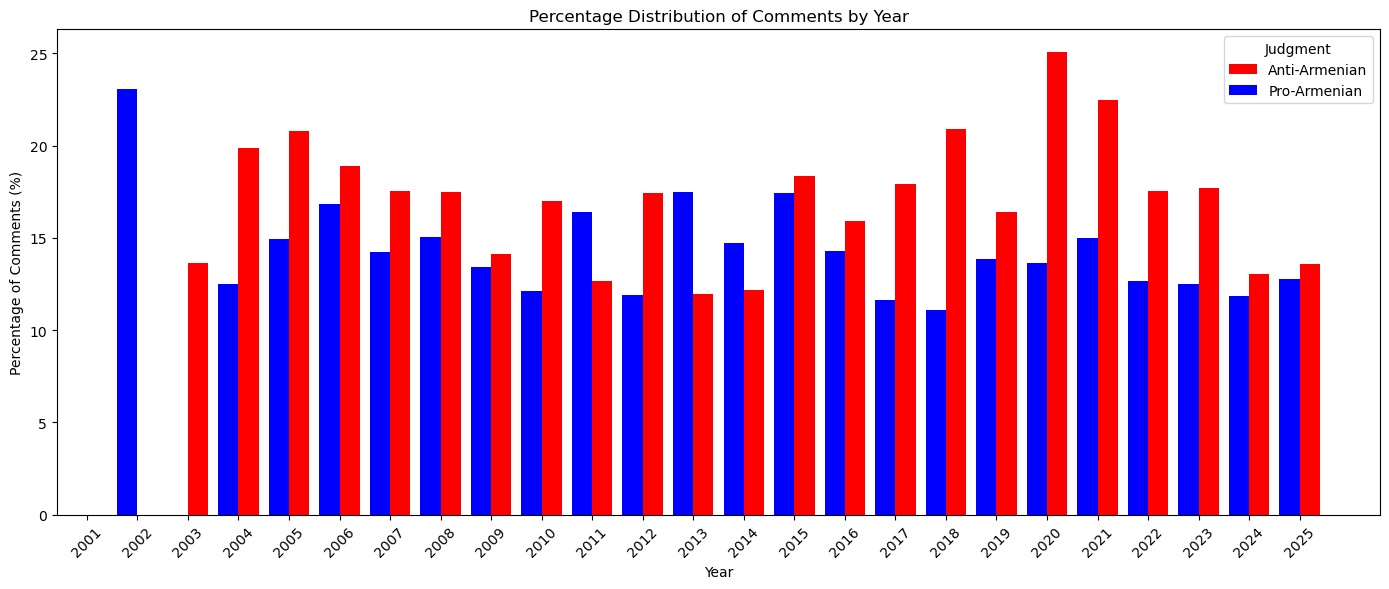
\includegraphics[width=0.8\linewidth]{fig/barplot_ratio.png}
    \caption{Per-Year Percentage of Pro- And Anti-Armenian Revisions on English Wikipedia Over Time}
    \label{fig:barplot_ratio}
\end{figure}


We observe that the counts of revisions in general - judged as weaponized or otherwise - experienced a spike in 2005 and 2006, plateaued dimly in subsequent years, only to then spike once more in the year 2020. It is also particularly clear that the share of Anti-Armenian revisions, compared to both Pro-Armenian revisions and Non-Weaponized revisions, noticeably spiked to its highest in the years 2020 and 2021 (at 25.04\% and 22.48\%, respectively) while the stats largely hovered around 16\% for all of the other years. No spike to such a noticeable degree was observed among Pro-Armenian revisions in 2020. We can plausibly attribute the spike in 2020 to the onset of the Second Nagorno-Karabakh War in September 2020 as Azerbaijani forces invaded the ethnically-Armenian Republic of Artsakh and massively reduced its territory, in what was a major escalation of the long-standing conflict between Armenia and Azerbaijan over the Nagorno-Karabakh region. Investigation of the distribution of sources in 2020 (Tables \ref{tab:pro-2020} and \ref{tab:anti-2020}), where the article Second Nagorno-Karabakh War occupy the top share among both Pro- and Anti-Armenian revision, appear to also corroborate this observation, since they reflect an apparent urgent need to participate in discourse and edits of the Second Nagorno-Karabakh War article in 2020 despite it only having been created that very same year. The relatively high shares of revisions for articles ``Republic of Artsakh'' and ``Shusha'' (the city of Shusha fell to Azerbaijani forces in their 2020 offensive) across both camps in 2020 also lends credence to this theory. No such overwhelming disparity existed among the 2006 edits (Tables \ref{tab:pro-2006} and \ref{tab:anti-2006}), apart from the article Armenian Genocide seeing a slight lead, making it more likely that the spike in 2006 in both camps was caused by increasing editorial activity on Wikipedia as the website furthered matured and was popularized across the internet. 

\subsubsection{Technique Differences of Pro-Armenian vs Anti-Armenian Revisions}

\begin{table}[h!]
\centering
\begin{tabular}{@{}lrr@{}}  % left-aligned, right-aligned, right-aligned
\toprule
\textbf{Category} & \textbf{Count} & \textbf{Percentage (\%)} \\
\midrule
Second Nagorno-Karabakh War & 64 & 40.25 \\
Republic of Artsakh & 9 & 5.66 \\
Shusha & 8 & 5.03 \\
Nagorno-Karabakh Conflict & 7 & 4.40 \\
Armenian Genocide & 6 & 3.77 \\
\bottomrule
\end{tabular}
\caption{Top five pages ranked by revision count among Pro-Armenian revisions within the year 2020}
\label{tab:pro-2020}
\end{table}

\begin{table}[h!]
\centering
\begin{tabular}{@{}lrr@{}}  % left-aligned, right-aligned, right-aligned
\toprule
\textbf{Category} & \textbf{Count} & \textbf{Percentage (\%)} \\
\midrule
Second Nagorno-Karabakh War & 170 & 58.22 \\
Republic of Artsakh & 22 & 7.53 \\
Armenian Genocide & 13 & 4.45 \\
Shusha & 11 & 3.77 \\
Dolma & 10 & 3.42 \\
\bottomrule
\end{tabular}
\caption{Top five pages ranked by revision count among Anti-Armenian revisions within the year 2020}
\label{tab:anti-2020}
\end{table}

\begin{table}[h!]
\centering
\begin{tabular}{@{}lrr@{}}  % left-aligned, right-aligned, right-aligned
\toprule
\textbf{Source} & \textbf{Count} & \textbf{Percentage (\%)} \\
\midrule
Armenian genocide & 73 & 30.93 \\
Nagorno-Karabakh & 31 & 13.14 \\
Armenia & 19 & 8.05 \\
Nakhchivan Autonomous Republic & 17 & 7.20 \\
First Nagorno-Karabakh War & 12 & 5.08 \\
\bottomrule
\end{tabular}
\caption{Top five pages ranked by revision count among Pro-Armenian revisions within the year 2006}
\label{tab:pro-2006}
\end{table}

\begin{table}[h!]
\centering
\begin{tabular}{@{}lrr@{}}  % left-aligned, right-aligned, right-aligned
\toprule
\textbf{Source} & \textbf{Count} & \textbf{Percentage (\%)} \\
\midrule
Armenian genocide & 75 & 28.30 \\
Nagorno-Karabakh & 36 & 13.58 \\
Nakhchivan Autonomous Republic & 27 & 10.19 \\
Armenia & 16 & 6.04 \\
First Nagorno-Karabakh War & 16 & 6.04 \\
\bottomrule
\end{tabular}
\caption{Top five pages ranked by revision count among Anti-Armenian revisions within the year 2006}
\label{tab:anti-2006}
\end{table}


Tables \ref{tab:ref-pro} and \ref{tab:ref-anti} presents the respective distributions of weaponization categories across all edits in the subdataset judged as "Pro-Armenian" and "Anti-Armenian", respectively:

\begin{table}[h!]
\centering
\begin{tabular}{@{}lrr@{}}  % left-aligned, right-aligned, right-aligned
\toprule
\textbf{Category} & \textbf{Count} & \textbf{Percentage (\%)} \\
\midrule
Terminology Biasing & 989 & 56.16 \\
Glorification \& Vilification & 254 & 14.42 \\
Selective Omission & 237 & 13.46 \\
Selective Insertion & 236 & 13.40 \\
Source Biasing & 15 & 0.85 \\
Tag Manipulation & 12 & 0.68 \\
Timeline Rewriting & 11 & 0.62 \\
Euphemism and Doublespeak & 5 & 0.28 \\
Citation Deletion & 2 & 0.11 \\
\bottomrule
\end{tabular}
\caption{Category distribution among the 1761 revisions annotated as Pro-Armenian.}
\label{tab:ref-pro}
\end{table}

\begin{table}[h!]
\centering
\begin{tabular}{@{}lrr@{}}  % left-aligned, right-aligned, right-aligned
\toprule
\textbf{Category} & \textbf{Count} & \textbf{Percentage (\%)} \\
\midrule
Terminology Biasing & 1006 & 45.75 \\
Selective Omission & 870 & 39.56 \\
Glorification \& Vilification & 183 & 8.32 \\
Selective Insertion & 65 & 2.96 \\
Euphemism and Doublespeak & 31 & 1.41 \\
Tag Manipulation & 29 & 1.32 \\
Source Biasing & 9 & 0.41 \\
Timeline Rewriting & 3 & 0.14 \\
Citation Deletion & 2 & 0.09 \\
Citation Washing & 1 & 0.05 \\
\bottomrule
\end{tabular}
\caption{Category distribution among the 2199 revisions annotated as Anti-Armenian.}
\label{tab:ref-anti}
\end{table}


Several insights can already be drawn from the observed distribution of revision-based weaponization tactics. First, \textbf{Terminology Biasing}, \textbf{Selective Omission}, and \textbf{Glorification \& Vilification} emerge by far as the most frequently employed techniques across Armenian-related English Wikipedia articles. Notably, this overall preference does not differ substantially between Pro-Armenian and Anti-Armenian revisions, suggesting a shared reliance on these mechanisms regardless of ideological stance.

Second, beyond variations that may plausibly be attributed to natural editorial noise, we observe a \textbf{markedly higher ratio of Selective Omission among Anti-Armenian revisions}. This asymmetry plausibly indicates a tendency within Anti-Armenian edits toward the removal of information in ways that may escape immediate detection by editors or readers, pointing to deletion rather than insertion as a comparatively “preferred” weaponization strategy within that camp.

Third, Pro-Armenian revisions display a corresponding affinity for \textbf{Selective Insertion}. One plausible explanation is that Armenian culture and history being the primary subject matter of the articles under study may encourage Pro-Armenian editors to adopt a more defensive or corrective posture, prompting the addition of contextual or supplementary information intended to emphasize Armenian historical contributions and/or suffering. The consistency of this pattern with intuitively expected editorial behavior lends further credence to the validity of the LLM-based categorization pipeline, both in terms of stance detection and weaponization technique classification.

Another important—if slightly less quantitatively pronounced—contrast between the two camps lies in their respective uses of \textbf{Glorification \& Vilification}. While such entries constitute a marginally smaller proportion of Anti-Armenian edits, the language employed in these revisions is, on average, significantly more crude, emotionally totalizing, and vitriolic than that observed in their Pro-Armenian counterparts.

For example, edits representative of Pro-Armenian revisions categorized under ``Glorification \& Vilification'' include:

\begin{itemize}
\item The added words ``turkey'', ``hide'', ``guilty'', ``of'', ``genocide'', ``shame'', ``on'', and ``obama'' create a strongly accusatory tone directed at Turkey regarding the Armenian Genocide. This phrasing explicitly assigns blame and implicates political leadership, shifting the edit from descriptive narration toward moral condemnation. [...]

\item The revision adds the phrase ``which he has not yet used'' to a sentence describing President George W. Bush’s annual April 24 speech. This addition introduces an evaluative dimension that highlights the President’s failure to explicitly acknowledge the Armenian Genocide, reframing an otherwise neutral statement as implicitly critical. [...]
\end{itemize}

By contrast, edits categorized as Anti-Armenian under the same technique frequently exhibit a higher density of overtly hostile and dehumanizing language, as illustrated by the following examples:

\begin{itemize}
\item The added line ``IT IS A BIG LIE AND LAST CHANGE FOR 'POOR ARMENIANS' TO GAIN THE MERCY OF ALL WORLD. THEY DO THAT FOR MONEY:)..You POOR ARMENIANS....!! HERE IS 5 Cents FROM ME :))'' employs mocking, derogatory phrasing while dismissing the historical reality of the Armenian Genocide. [...]

\item The removed line ``Armenians: see dirty, ugly, hairy, poor, disgusting food.'' contains explicitly demeaning and dehumanizing descriptors directed at Armenians. [...]
\end{itemize}

These qualitative differences align with broader expectations regarding discourse surrounding Armenian history and culture, where Anti-Armenian voices may be more inclined toward overtly combative or contemptuous rhetorical strategies. This further underscores the importance of examining the \emph{content and tone} of revisions beyond their categorical labels in order to meaningfully assess the nature of ideological weaponization. While we currently refrained from introducing a distinct ``Slurs \& Insults'' category—on the grounds that such edits could be subsumed under Glorification \& Vilification in their shared use of emotionally charged, factually unsubstantiated language—the above observations indicate that such a distinction may be warranted in future taxonomies.

\subsection{Implications for Wikipedia Moderation}

Beyond methodological considerations, the behavioral patterns observed in weaponized revisions carry several implications for Wikipedia moderation practices. First, our findings support DHLab's past study on the Russo-Ukrainian War in that a substantial proportion of narrative manipulation operates through \emph{procedurally legitimate} edits—such as selective omission, terminology biasing, and tag manipulation—rather than through overt vandalism or easily detectable abuse. These edits often remain formally compliant with Wikipedia’s policies while nonetheless exerting cumulative ideological influence, making them particularly difficult to identify through rule-based moderation alone.

Second, the asymmetry in preferred weaponization strategies across factions highlights a blind spot in current moderation workflows. Anti-Armenian revisions disproportionately rely on selective omission, a tactic that is inherently harder to flag than inflammatory insertions because it removes context rather than adding explicit claims. In contrast, Pro-Armenian revisions more frequently employ selective insertion and overt evaluative language, which may attract greater scrutiny precisely because they are more visible. This asymmetry suggests that moderation systems—both human- and tool-assisted—has the possibility to inadvertently penalize certain forms of bias while systematically overlooking others.

Third, the qualitative differences in the use of Glorification \& Vilification indicate that not all emotionally charged edits are equivalent in tone or severity. While both camps engage in evaluative framing, Anti-Armenian revisions more frequently employ crude, dehumanizing, or explicitly hostile language. The fact that such edits are currently subsumed under broader categories points to the potential utility of finer-grained moderation signals that distinguish between rhetorical intensity levels rather than treating all emotional framing uniformly.

Finally, the temporal clustering of weaponized edits around moments of real-world conflict—most notably the 2020 Nagorno-Karabakh War—suggests that Wikipedia moderation efforts may benefit from \emph{context-aware escalation mechanisms}. Periods of geopolitical crisis correspond to spikes in factional editing activity, implying that static moderation thresholds may be insufficient during high-risk intervals. LLM-assisted monitoring pipelines, such as the one explored in this study, could support moderators by flagging subtle but systematic narrative shifts during these periods, rather than reacting solely to individual high-profile disputes.


\section{Limitations and Future Work}

A primary observation shared across all experiments is that LLMs—specifically \texttt{4o-mini}—appear reasonably effective at distinguishing between weaponized and non-weaponized revisions, as well as between Pro-Armenian and Anti-Armenian stances among weaponized instances, in an intuitively coherent manner. That said, \texttt{4o-mini}, like LLMs in general, is \textbf{not immune to miscategorization}.

One illustrative failure case involves four revisions containing the phrase ``TAKE AWAY THE TURKISH FLAGS FROM THE GREEK ISLANDS !! SHAME ON YOU !! YOU ARE NOT OBJECTIVE !!!!'', which the pipeline misclassified as Anti-Armenian despite the clearly anti-Turkish sentiment being explicitly included in the Pro-Armenian stance definition provided to the model. While such cases remain relatively rare—accounting for only 8 misclassified revisions (4.4\%) among the 183 Anti-Armenian Glorification \& Vilification instances—they nevertheless demonstrate that classification errors are not entirely negligible.

This highlights the need for future work aimed at reducing LLM-driven misclassification in any prospective fully automated pipeline intended to monitor and categorize Wikipedia edits related to Armenian culture and history in real time. In the near term, this could be addressed through fine-tuning smaller, lower-parameter models trained specifically for this task, or through the deployment of a more traditional BERT-based classifier. Either approach would require comprehensive manual annotation—at minimum across the subsampled 12,659-revision dataset—using the ten-category weaponization taxonomy developed in this study.

Beyond technical limitations, a more conceptual constraint of this work lies in the inherently human-influenced and somewhat arbitrary nature of defining what constitutes cultural weaponization in the first place. Distinguishing between good-faith contribution and manipulative or malicious edits is often nontrivial, particularly given that revision diffs rarely provide information about factual verifiability, especially for newly added material. 
One may also question whether emotionally charged language itself constitutes a weaponized tactic, or even falls within the realm of framing techniques in general. Pastorino et al., for example, argued in their study on LLM detection of framing techniques in news headlines that, at least within the domain of news headlines, emotional expression in itself is fundamentally distinct enough from deliberate framing \cite{pastorino2024decodingnewsnarrativescritical}. This ambiguity inevitably shapes both human annotation and - further downstream - LLM-based classification outcomes.

Accordingly, future studies on Wikipedia cultural vandalism and ideological manipulation are encouraged to explore alternative definitions, taxonomies, and stance frameworks, and to assess whether similar patterns emerge across Armenian-related content under differing conceptualizations of weaponization.

\section{Conclusion}

This study demonstrates that revision-level analysis, when combined with LLM-assisted reasoning, offers a viable and effective approach for detecting and categorizing cultural heritage weaponization on Wikipedia. Through a large-scale case study on Armenian-related articles, we show that unsupervised clustering and topic modeling alone struggle to disentangle manipulation techniques from topical content, whereas LLM-based classification enables the construction of a refined, technique-oriented taxonomy grounded in empirical editorial behavior. The resulting ten-category taxonomy captures a wide spectrum of subtle yet impactful manipulation strategies that frequently evade traditional vandalism detection frameworks.

Beyond methodological insights, our findings reveal asymmetric editorial behaviors across ideological camps, temporal spikes in weaponization activity aligned with real-world conflict, and systematic reliance on procedurally legitimate but narratively manipulative edits. These observations underscore the limitations of existing moderation paradigms and reaffirm the potential of LLM-assisted pipelines as decision-support tools for large-scale, context-aware monitoring. More broadly, this work suggests that understanding how cultural narratives are contested at the level of individual revisions is essential for preserving the integrity of collaborative knowledge platforms in politically and historically sensitive domains.

\printbibliography

\end{document}
